\documentclass{article}
\usepackage{graphicx}
\usepackage[utf8]{inputenc}
\usepackage[french]{babel}
\usepackage{xcolor}
\usepackage[a4paper, total={6in, 8in}]{geometry}
\title{Projet GraphMining}
\author{emeric.l }
\date{December 2023}

\begin{document}


\begin{titlepage}
\newcommand{\HRule}{\rule{\linewidth}{0.5mm}}
\center


\includegraphics[width=6cm]{assets/logo_unamur}
\\[2cm]

\textsc{\LARGE Université de Namur}
\\[2cm]

\textsc{\Large SDASM101 : Graph mining }
\\[0.2cm]

\HRule
\\[0.4cm]
\textsc{\huge Projet : Analyse des données}
\\[0.2cm]
\HRule
\\[0.4cm]
{\large 2023 - 2024}
\\[8.2cm]

\begin{minipage}{0.5\textwidth}
	\begin{flushleft}
		\emph{Auteur}
		\\
		\textsc{Lambois} Emeric
		\\
		\textsc{Santelé} Victor
		\\
		\textsc{Smith} Jonathan
		\\
	\end{flushleft}
\end{minipage}
~
\begin{minipage}{0.4\textwidth}
	\begin{flushright}
		\emph{Professeur}
		\\
		\textsc{Salnikov} Vsevolod
		\\
	\end{flushright}
\end{minipage}

\end{titlepage}

\tableofcontents
\newpage

\section{Introduction}

Dans le cadre du cours de « Graph Mining », il était attendu que chaque groupe se focalise sur l’étude des graphes empiriques, sous différentes facettes. C’est pourquoi, les objectifs attendus lors de la réalisation de ce projet sont de manipuler les concepts établis lors des différentes séances de cours que nous avons eu. De plus, il nous est demandé de comparer 2 graphes provenant de « sociopatterns.org » et de les comparer de sorte que les différentes techniques vues au cours soient appliquées.

\section{Jeu de données}

Dans l'objectif de mener à bien le projet, nous avons opté pour l'utilisation de deux ensembles de données présents dans la base de données mise à notre disposition par le professeur. Ainsi, nous avons convenu de sélectionner deux ensembles qui nous semblaient pertinents. \\

C'est la raison pour laquelle nous avons choisi, en premier lieu, les données relatives aux contacts entre employés d'une entreprise pour l'année 2013. Cet ensemble de données représente le réseau temporel des interactions entre individus mesurées dans un immeuble de bureaux en France, du 24 juin au 3 juillet 2013. \\

En tant que deuxième ensemble de données, nous avons sélectionné les contacts entre employés d'une entreprise pour l'année 2015. Ces données comprennent le réseau temporel des contacts entre individus mesurés dans un immeuble de bureaux en France au cours de l'année 2015.

\section{Propriétés de Base du Graphe}

Dans cette section, nous allons examiner les caractéristiques fondamentales des deux graphes que nous avons sélectionnés.

\subsection{Noeuds et arêtes}

\noindent
Nous allons commencer par explorer les nœuds et arêtes de ces deux graphes. \\

Effectivement, pour chaque graphe, tous les nœuds présents dans ces graphes représentent un employé et chaque arête de ces graphes représente un contact entre deux employés. \\

Dans la première partie de cette analyse graphique, nous plongeons dans un ensemble de données composé de 92 nœuds représentant des employés et de 755 arêtes représentant les contacts entre eux au cours de l'année 2013. La densité de 0.1804 indique que seulement 18,04 \% des connexions potentielles sont établies dans ce réseau. Cette faible densité suggère une certaine rareté dans les interactions entre collègues. Il se pourrait que cette dynamique soit influencée par la structure organisationnelle spécifique mise en place en 2013. \\

La seconde partie, en 2015, contient un ensemble de données plus vaste. Car il compte 217 nœuds et 4 274 arêtes, formant un réseau complexe. La densité de 0.1824, bien que légèrement supérieure à celle de 2013, indique que 18.24 \% seulement des connexions potentielles est active dans ce réseau. Les interactions au sein de ce réseau mettent en lumière l’échange plus dynamique de la communication interne. \\

Ainsi, notre exploration dévoile non seulement des chiffres et des liens, mais aussi les nuances subtiles d'une communication interne façonnée par la dynamique organisationnelle.

\subsection{Distribution du Degré}

En ce qui concerne la distribution de ceux-ci, nous pouvons voir que la moyenne et la médiane du graphe de 2013 étant proches, cela suggère une distribution symétrique.
Nous pouvons aussi voir que certains nœuds sont très connectés et cela est vérifié par le fait que le quartile 90e est plus élevé que la moyenne. Cela peut être interprété par des employés possédants un poste potentiellement plus important, socialement poussant alors à créer plus de contact avec d’autres employés. \\

Ensuite, nous pouvons également voir que pour le graphe de 2015, la distribution suggérée semble être aussi symétrique. Nous pouvons aussi apercevoir que ces graphes possèdent aussi des nœuds très connectés. Cette augmentation du nombre de nœuds ainsi que le nombre de nœuds fortement connecté suggèrent probablement une simple à croissance de l’entreprise donnant lieu à plus de postes à haute importance sociale, comme des chefs d’équipe par exemple, en multipliant le nombre d’équipe présente dans la société.

\begin{figure}[!h]
    \centering
    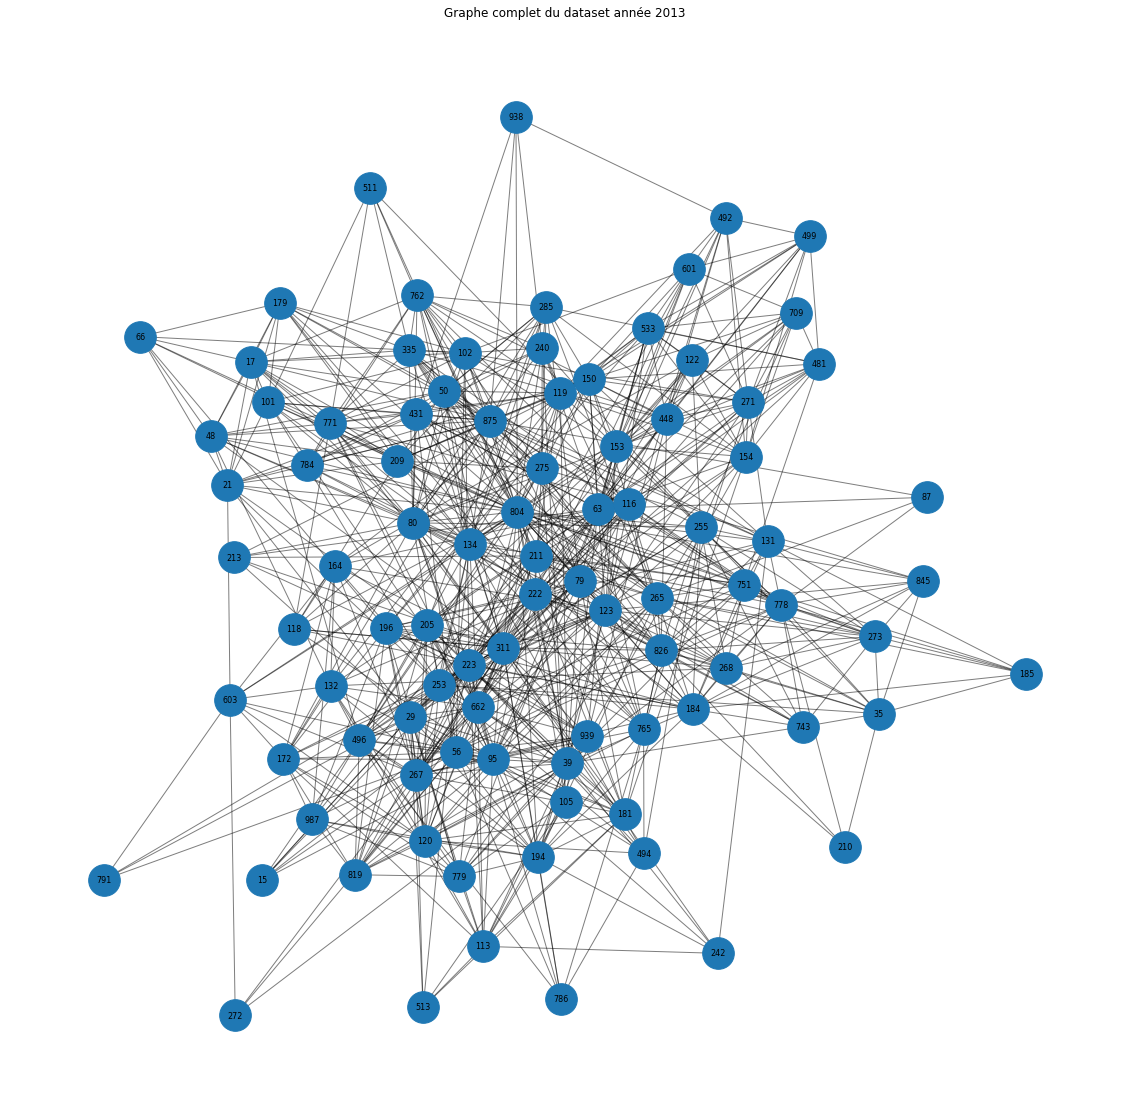
\includegraphics[width=0.45\textwidth]{assets/proprietebase/2013}
    \hfill
    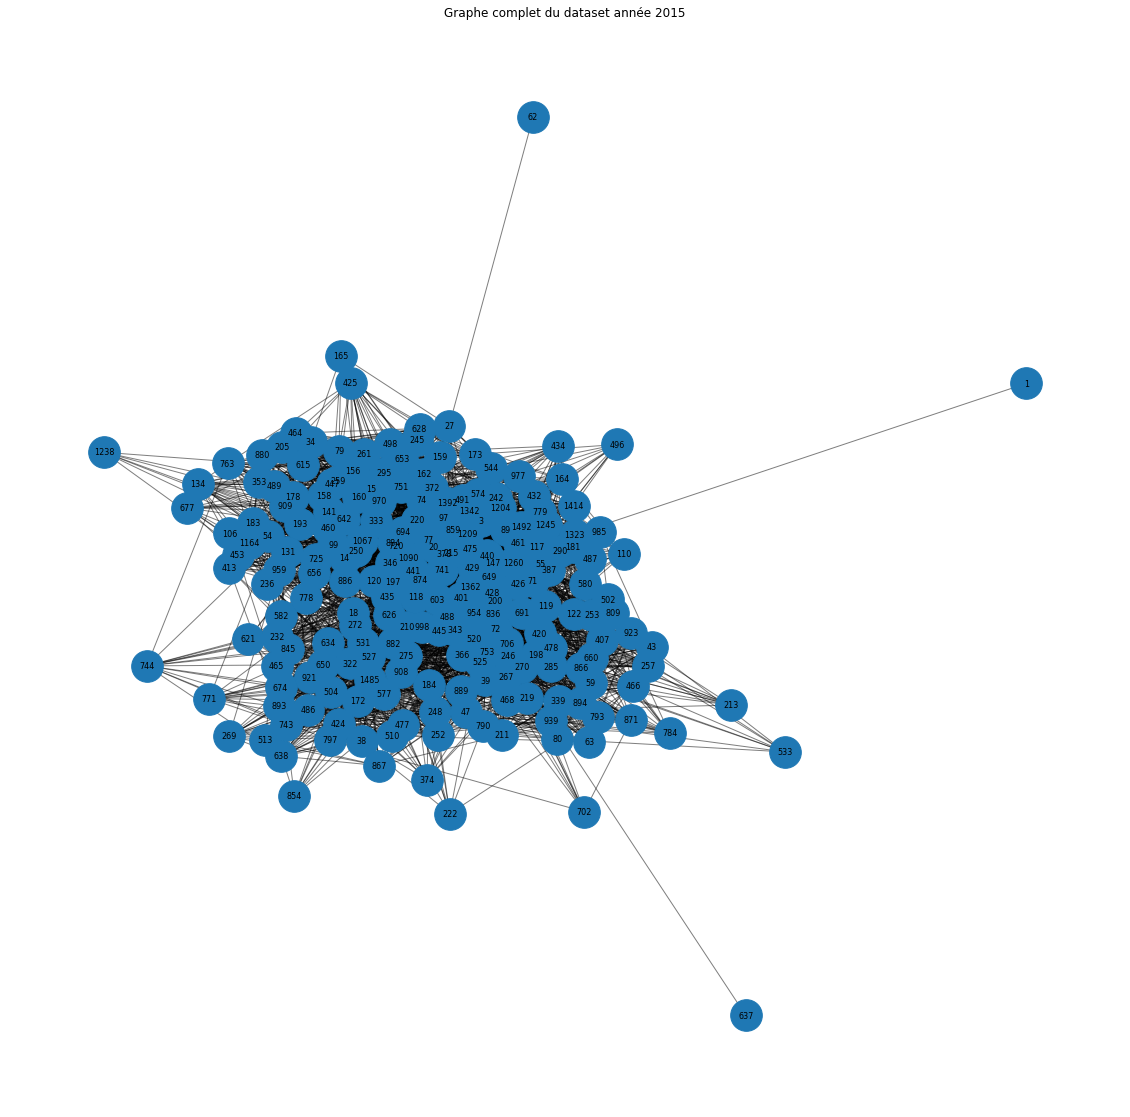
\includegraphics[width=0.45\textwidth]{assets/proprietebase/2015}
    \caption{Graphes des années 2013 et 2015}
    \label{fig:2013-2015}
\end{figure}

\section{Modèle épidémiologie}

Maintenant, que l'introduction aux graphes est terminée, essayons de mettre à l'épreuve les employés en simulant la propagation d'une maladie.

\subsection{Centres de Propagation}

Commençons par définir les centres de propagation. Dans nos graphes, ces centres correspondent en réalité aux noeuds fortement connectés, ceux qui présentent le plus haut degré de connexion. Comme mentionné précédemment, il est possible que ces nœuds représentent des postes à haute responsabilité au sein de la société. En ce qui concerne le premier graphe (Année 2013), la figure ci-dessous illustre les différents noeuds fortement connectés. Nous pouvons voir à travers cette illustration que les noeuds sont très souvent proche du centre du graphe de pars leurs forte connexion avec le reste des noeuds.

En ce qui concerne le deuxième graphe (Année 2015), la figure ci-dessous illustre les différents noeuds fortement connectés. Ici, l'illustration met évidence que ces noeuds fortement connecté se situent également proche du centre de la majorité des connexion.

Il est intéressant de noter que cette disposition renforce l'idée que les nœuds centraux jouent un rôle clé dans la dynamique des connexions au sein de l'ensemble du réseau.

\begin{figure}[!h]
    \centering
    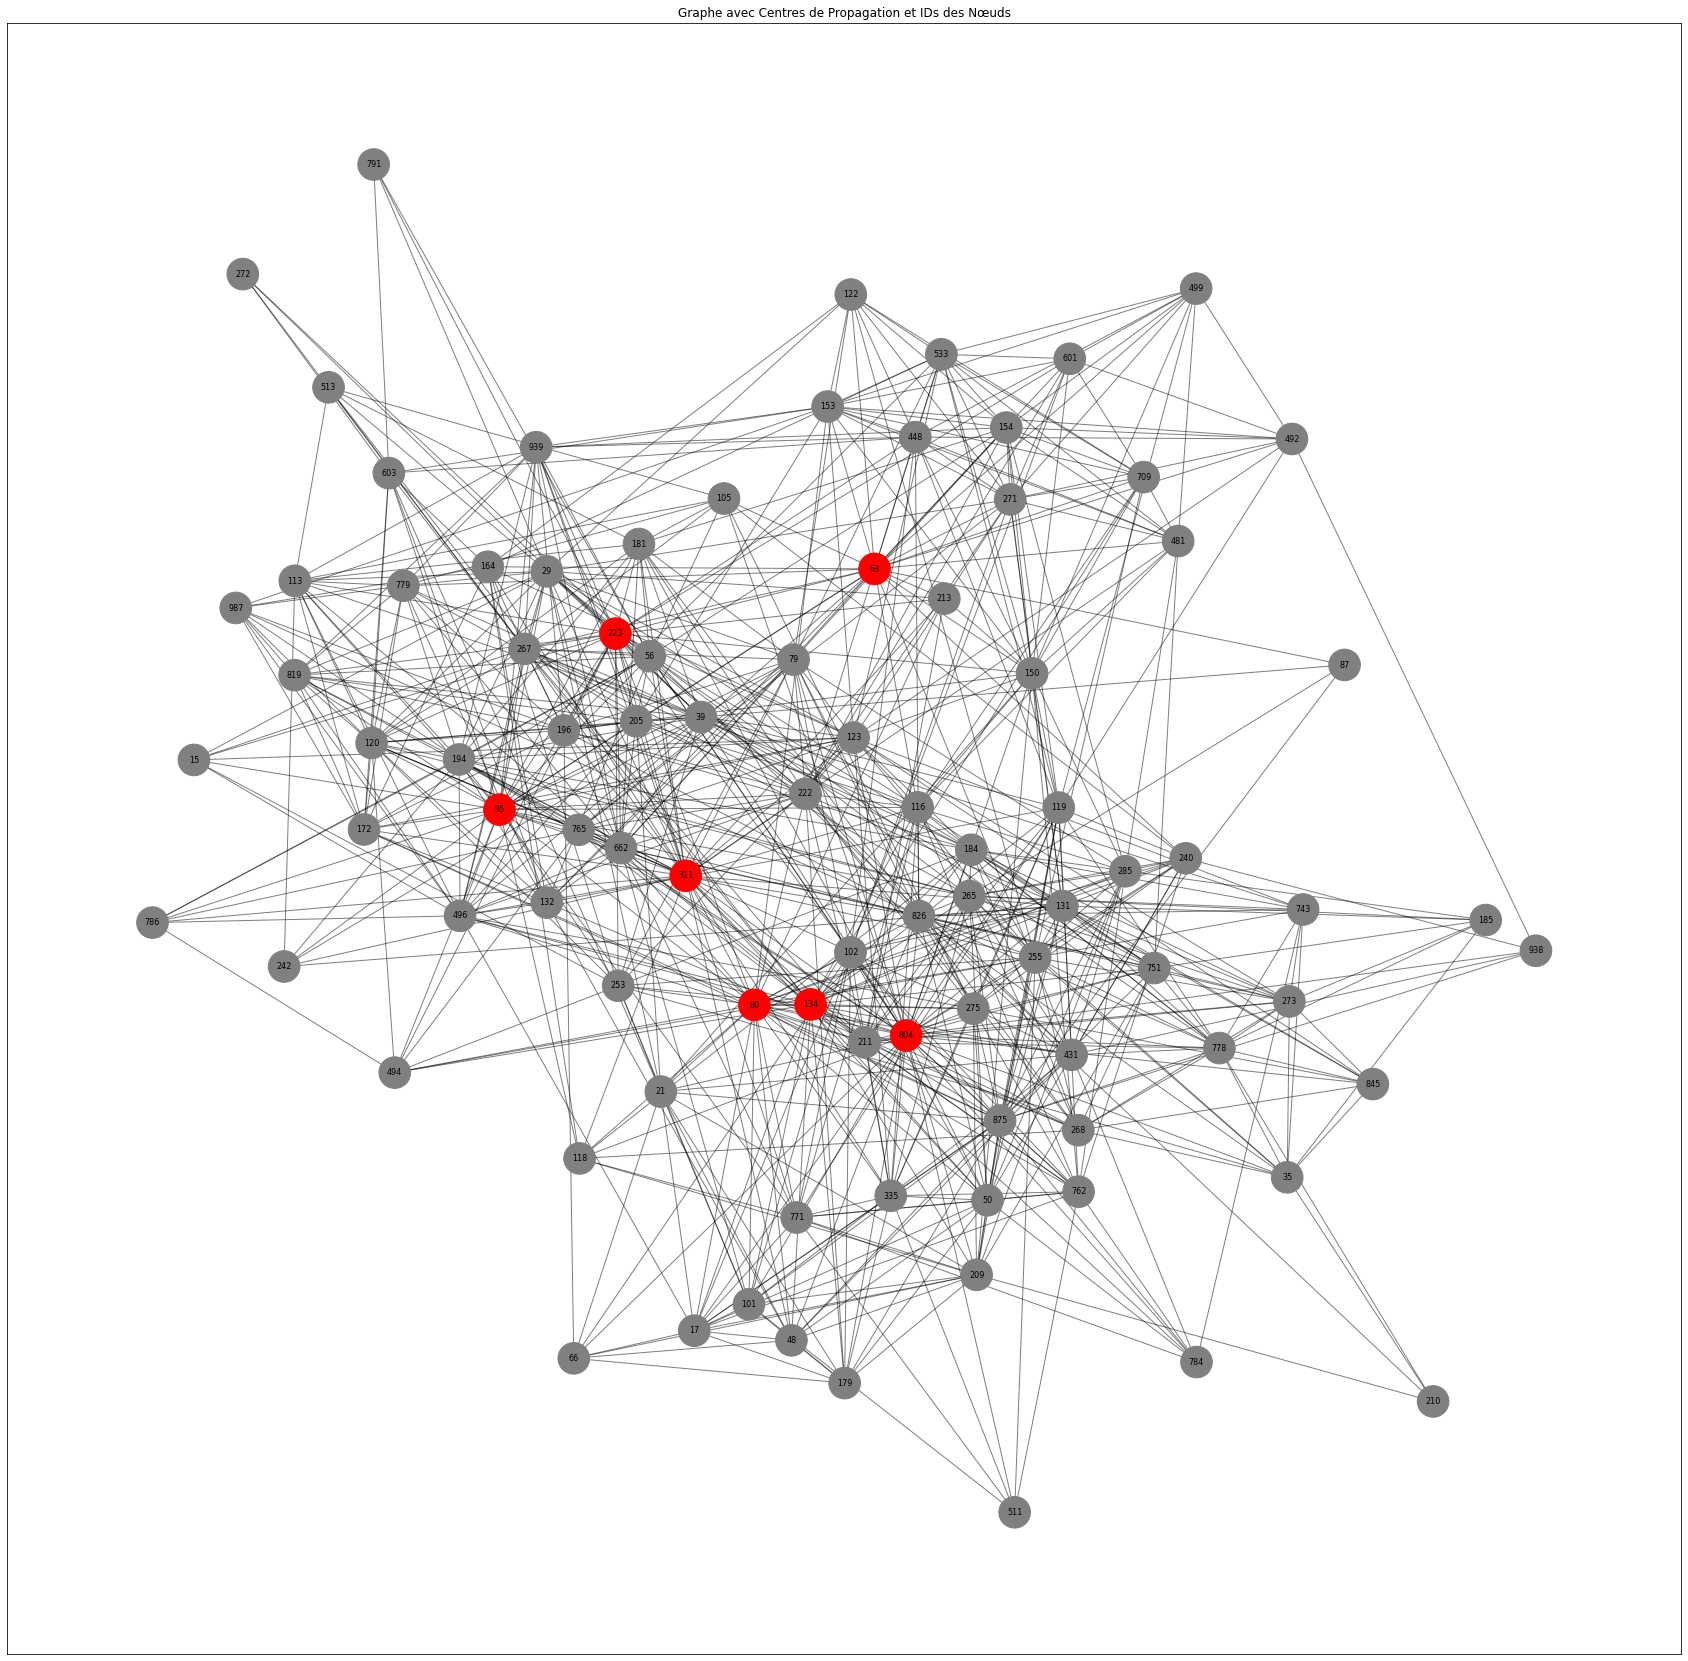
\includegraphics[width=0.45\textwidth]{assets/epidemiologie/centre_propa_2013}
    \hfill
    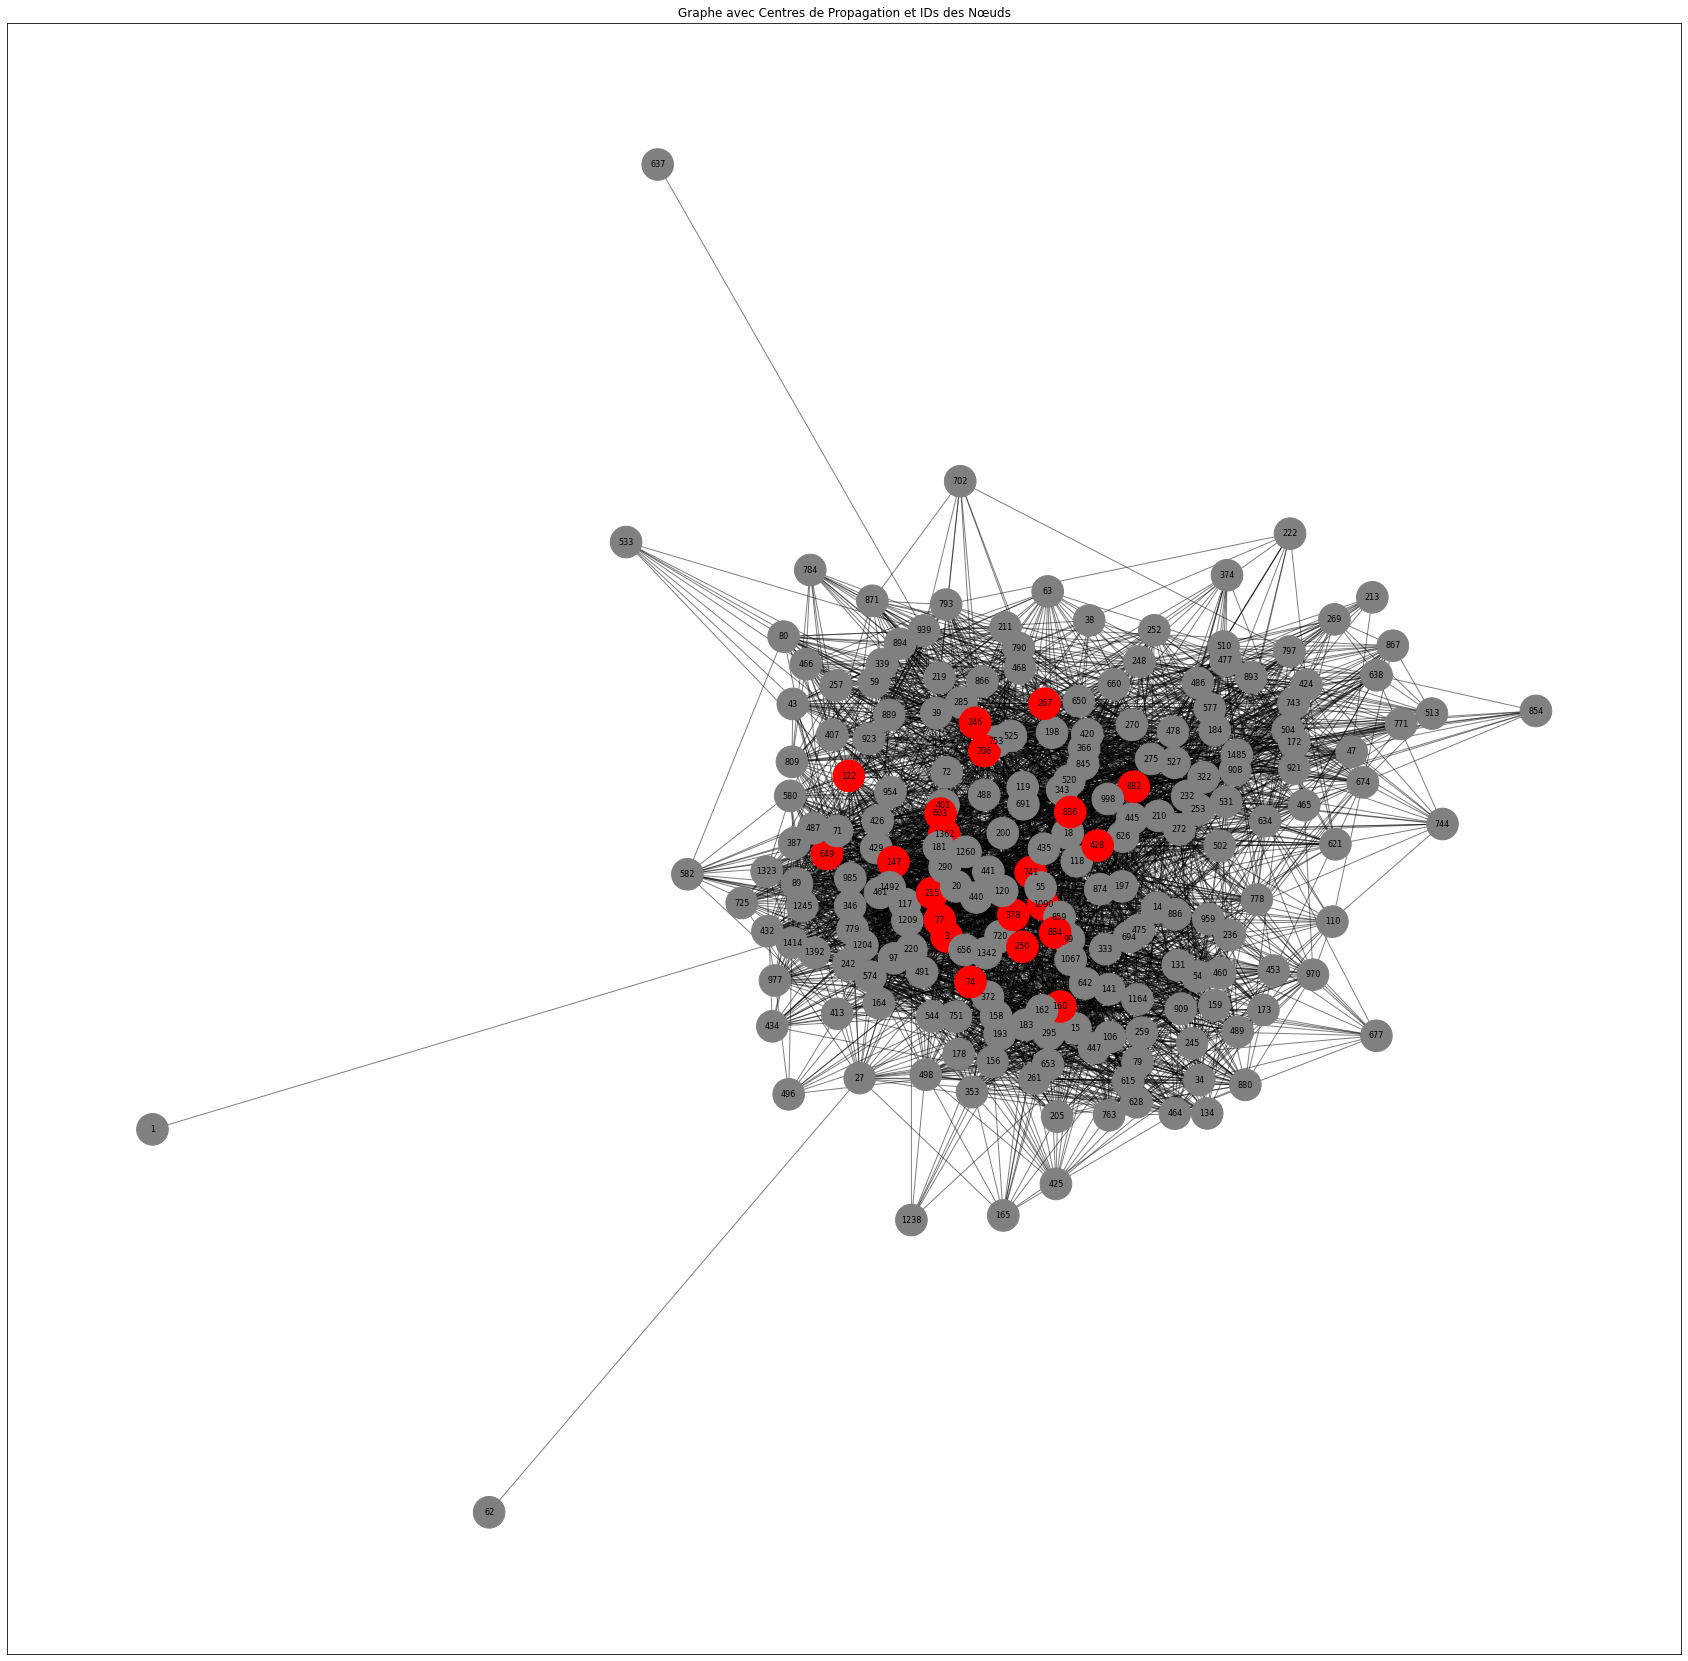
\includegraphics[width=0.45\textwidth]{assets/epidemiologie/centre_propa_2015}
    \caption{Centres de propagations pour les années 2013 et 2015}
    \label{fig:centre_propa_parallel}
\end{figure}

\clearpage
\newpage
\subsection{Seuils de Propagation}

\noindent
Dans le but de propager l'épidémie, nous avons défini deux paramètre :
\begin{itemize}
    \item beta : Taux de transmission, qui détermine la probabilité qu'un nœud susceptible devienne infecté lorsqu'il est en contact avec un nœud infecté.
    \item gamma : Taux de récupération, qui indique la probabilité qu'un nœud infecté récupère et devienne immunisé. \\
\end{itemize}

Ces deux paramètres servent simplement de taux d'influences pour le comportement du modèle épidémique. Ajuster ces valeurs permet de changer la propagation de la maladie.

Nous les avons ajusté à :
\begin{itemize}
    \item beta = 0.3 (Taux de transmission)
    \item gamma = 0.1 (Taux de récupération)
\end{itemize}


Nous avons décidé de mettre à l'épreuve cette société en y incluant un collaborateurs infecté afin de voir comment se propagerait une épidémie. C'est pourquoi, nous avons créé un petit scénario pour illustrer cela. \\

Lors d'un voyage d'affaire contenant l'intégralité des personnes à haute responsabilité dans l'entreprise, l'un des collaborateurs, sans le savoir, a contracté un virus insidieux pendant son voyage. À son retour au bureau, les premiers symptômes sont apparus, mais malheureusement, la nature légère des symptômes a conduit à un sous-estimation de la situation. Le virus, invisible et trompeur, s'est rapidement propagé au sein des bureaux de l'entreprise. \\

Les espaces de travail ouverts, les salles de réunion animées et les pauses-café conviviales ont été des terrains fertiles pour la transmission du virus. En un rien de temps, plusieurs employés ont été touchés, créant un climat d'incertitude et de préoccupation parmi les équipes.

\subsection{Simulation de Propagation}

Dans le but de simuler la propagation, nous avons utilisé le modèle SIR.

\textcolor{red}{En lien, la simu changera en fonction du déclenchement de l'épidémie}

\section{Détection de communautés}

Dans cette section, notre objectif est d'identifier la présence de communautés au sein de nos graphes en exploitant principalement la bibliothèque Python Louvain Community.

\subsection{Communautés}

Afin de détecter les communautés au sein de l'entreprise, notre approche initiale consiste à identifier les nœuds étroitement liés qui pourraient former une sous-population distincte au sein de la population globale d'employés. Cette sous-population, représentée comme une communauté d'employés, pourrait potentiellement correspondre à une équipe spécifique au sein de l'entreprise. \\

Pour cette raison, nous avons créé un graphique en barres (barplot) illustrant la distribution des degrés pour chaque nœud (employé). Ce graphique permet d'estimer dans un premier temps si le graphe présente des nœuds avec des degrés élevés. Nous débutons cette analyse en visualisant le graphe de l'année 2013, qui compte moins d'employés. \\

Dans ce premier graphe, nous observons une propension marquée à avoir un degré de 15, avec 13 nœuds. Cependant, nous constatons également que le nombre de nœuds ayant moins de 10 degrés est relativement faible. Il est important de noter l'existence de nœuds avec plus de 30 degrés, suggérant probablement qu'il s'agit de nœuds fortement connectés occupant des postes à haute responsabilité, comme mentionné précédemment. La moyenne des degrés s'élève à 16.41.

\begin{figure}[!h]
    \centering
    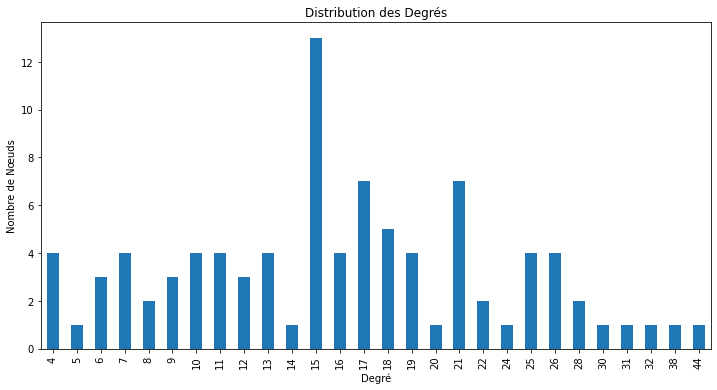
\includegraphics[width=0.65\textwidth]{assets/communaute/distribution_deg_2013}
    \caption{Distribution des degrés pour le graphe 1 de l'année 2013}
    \label{fig:distribution_deg_2013}
\end{figure}

Dans le deuxième graphe représentant l'année 2015, nous observons une moyenne presque deux fois plus élevée, soulignant une augmentation significative du nombre de connexions entre les employés. De plus, le degré maximal atteint 84, dépassant le maximum de 44 observé précédemment. Le nombre d'employés avec plus de 30 degrés est également majoritaire. \\

Ces observations suggèrent une amélioration potentielle de l'entreprise, tant en termes d'expansion du nombre d'employés que de qualité organisationnelle de la communication entre ces employés.


\begin{figure}[!h]
    \centering
    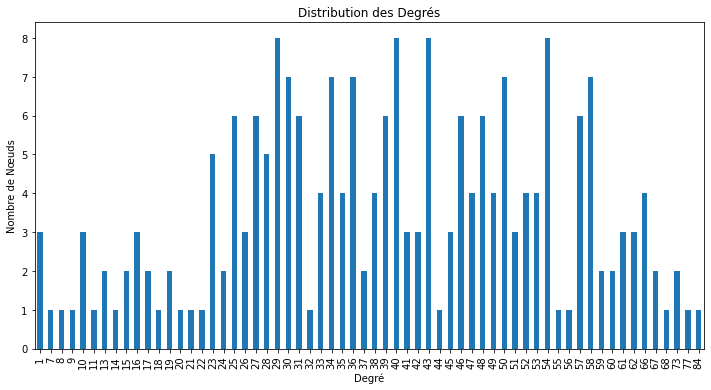
\includegraphics[width=0.65\textwidth]{assets/communaute/distribution_deg_2015}
    \caption{Distribution des degrés pour le graphe 1 de l'année 2015}
    \label{fig:distribution_deg_2015}
\end{figure}

\subsection{Détecter les Communautés}

Dans l'optique de déterminer de manière définitive les communautés au sein de nos graphes, nous avons utilisé la bibliothèque Louvain Community Detection, qui s'est avérée être un outil extrêmement efficace à cet égard. Cette approche nous a permis de gagner considérablement en temps et de parvenir à des résultats concluants. \\

Suite à la génération du graphe pour l'année 2013, nous avons identifié quatre communautés distinctes au sein de notre population globale. À première vue, il semblait que ces communautés correspondaient à des départements spécifiques au sein de l'entreprise, à savoir SFLE, DSE, SRH, DMCT et DISQ. \\

Cependant, un examen plus approfondi a révélé une nuance intéressante. Certains employés d'autres départements se retrouvent également dans certaines communautés comme des membres de DISQ qui se retrouvent avec des DMCT et DSE dans la première communauté. 


\begin{figure}[!h]
    \centering
    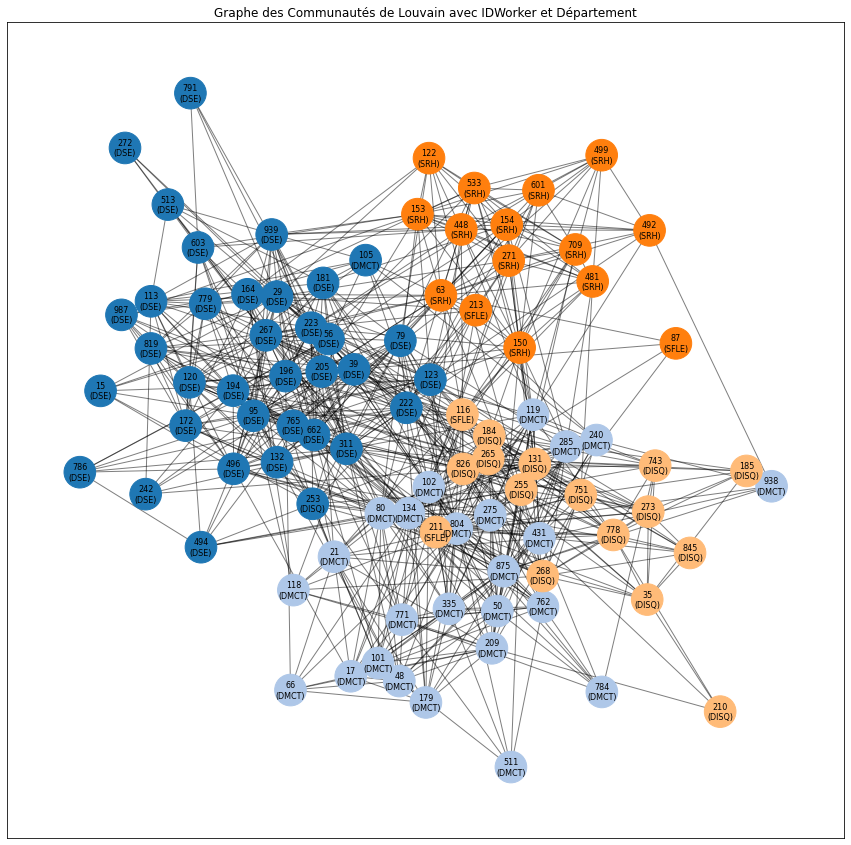
\includegraphics[width=0.45\textwidth]{assets/communaute/communaute_2013.png}
    \hfill
    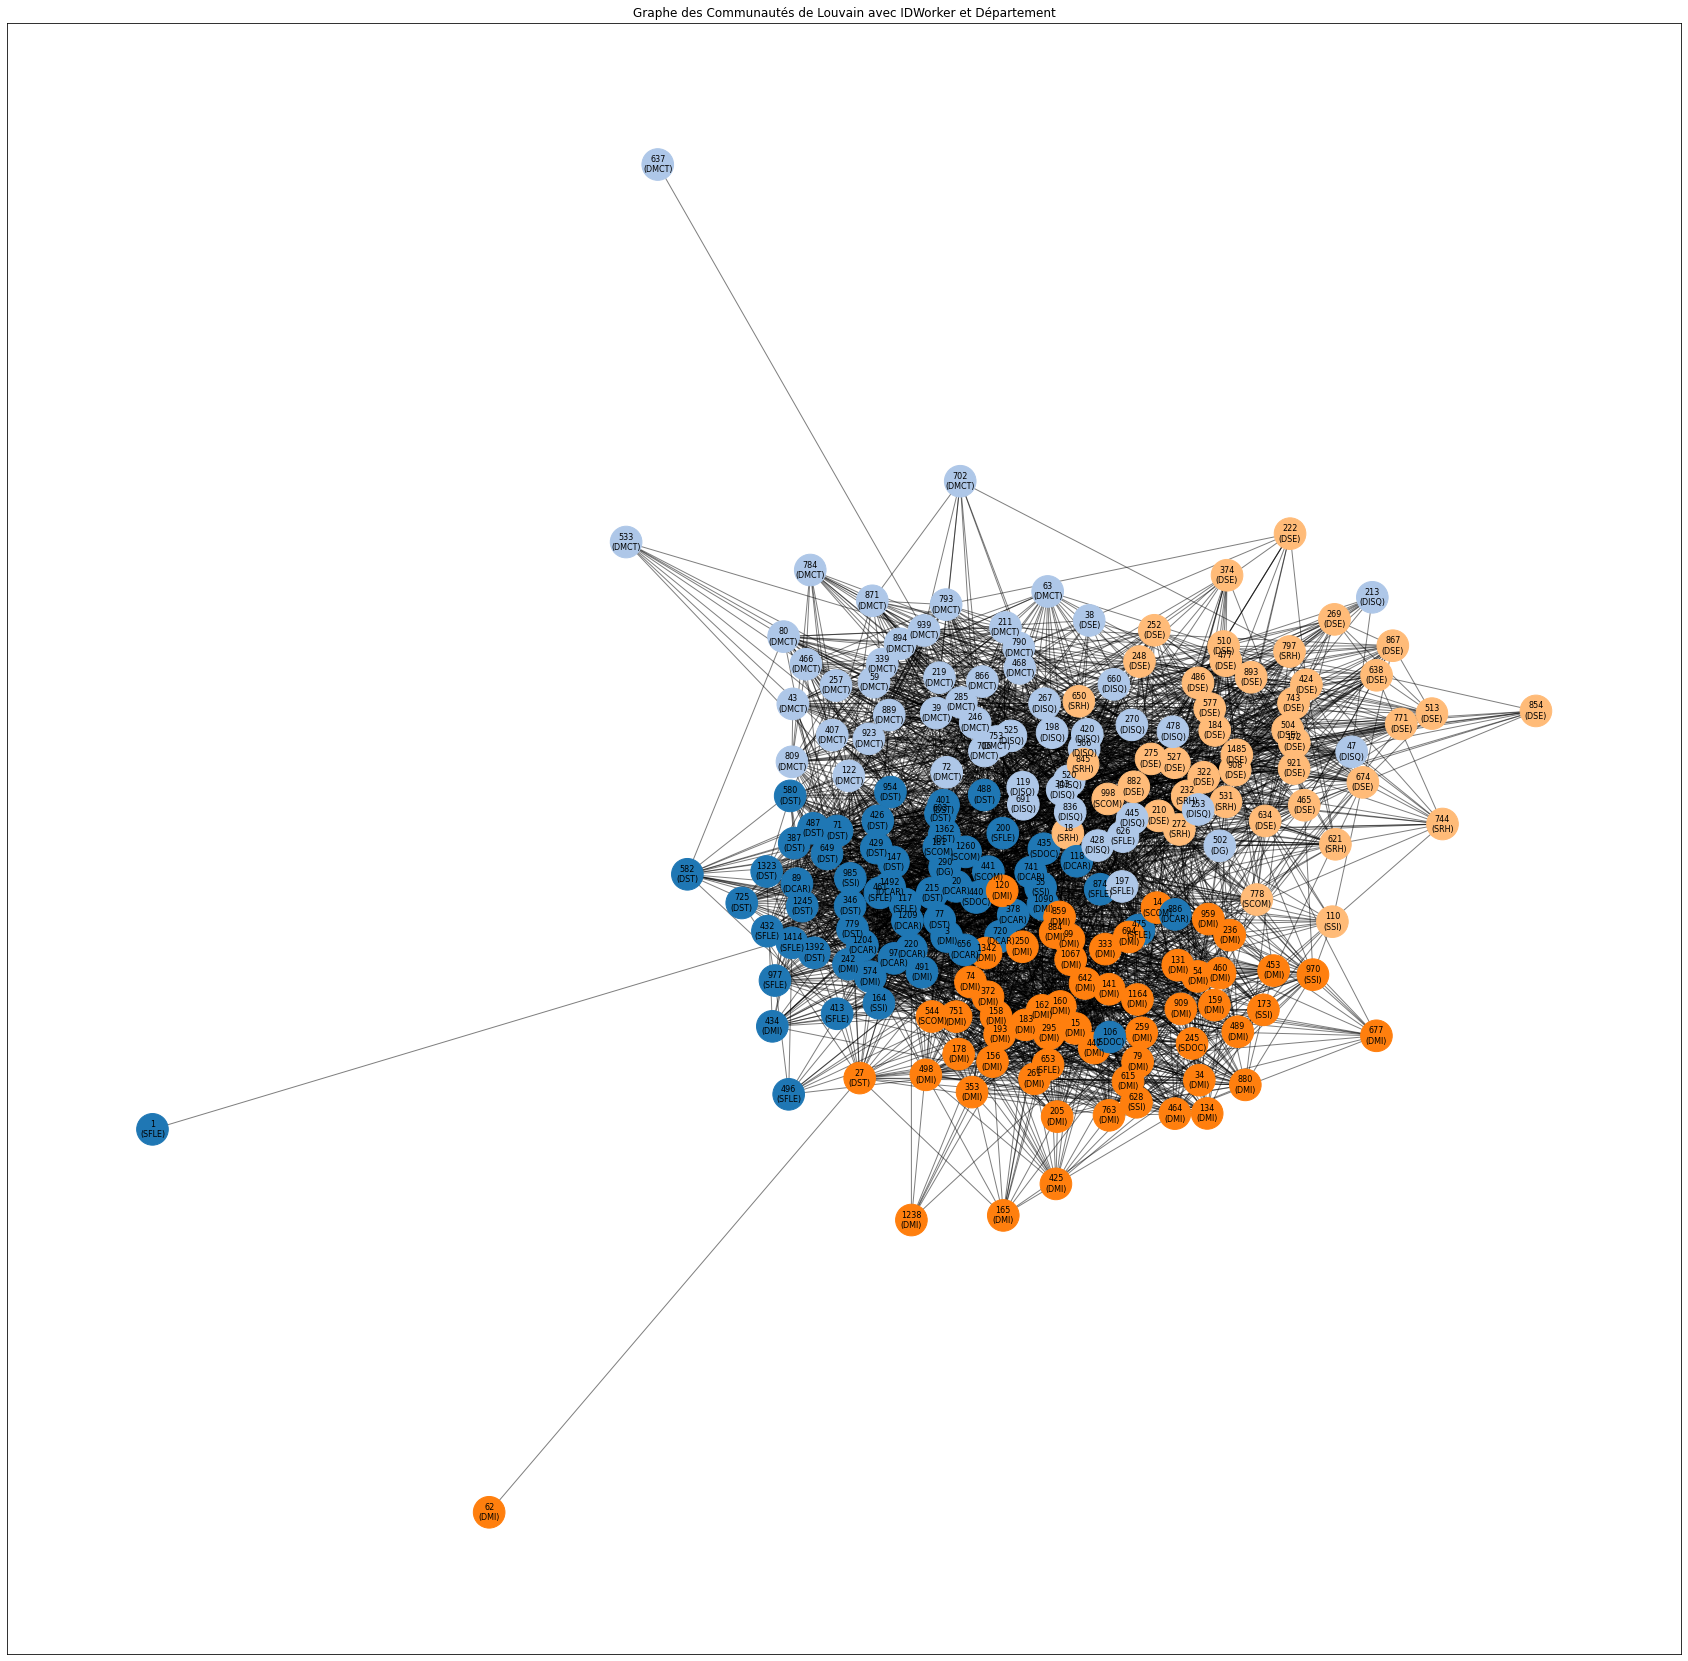
\includegraphics[width=0.45\textwidth]{assets/communaute/communaute_2015.png}
    \caption{Graphes des différentes communautés pour les années 2013 et 2015}
    \label{fig:communaute_parallel}
\end{figure}


Concernant l'année 2015, les résultats ont été un peu plus surprenants. Bien que nous ayons toujours identifié 4 communautés, la présence de différents départements est cette fois plus marquée. On aurait pu penser à des employés "hybrides", couvrant deux départements, mais cela ne semble pas être le cas. \\

En effet, on observe une augmentation du nombre de départements, passant de 4 en 2013 à 12 en 2015, à savoir SFLE, DMI, DST, DCAR, DG, SSI, SDOC, SCOM, DMCT, DISQ, DSE, SRH. Une hypothèse plausible serait que ces différentes communautés représentent des équipes travaillant sur divers projets. \\

\subsection{Analyse des Communautés}

En effet, comme mentionné précédemment, il semble que les communautés ne représentent pas nécessairement la répartition des employés dans les différents départements, contrairement à ce que pourrait laisser penser le graphe de 2013. Le graphique de 2015 révèle plutôt une diversité plus marquée dans la distribution des départements au sein des communautés. \\

L'hypothèse la plus plausible serait alors une répartition des employés au sein des différentes équipes de projet, composées de plusieurs départements. Cela pourrait être le cas, par exemple, avec des départements informatiques, économiques et juridiques travaillant en collaboration sur un projet complexe. \\

Nous avons également examiné l'évolution des communications au sein des différents départements pour évaluer si l'organisation communicationnelle a connu des changements. \\

Comme illustré dans le graphique ci-dessous (année 2013), nous observons cinq départements, chacun représenté par une boucle symbolisant la communication interne au sein du département. Cette visualisation permet d'évaluer la qualité de la communication interne de chaque département. Nous constatons que certains départements, tels que DES, DISQ, SRH et DMCT, présentent une communication interne solide. Cependant, les départements avec un effectif plus restreint affichent une communication interne plus faible. De plus, la visualisation révèle des liens de communication interdépartementaux forts, comme c'est le cas entre les départements DES et DISQ, par exemple.

\begin{figure}[!h]
    \centering
    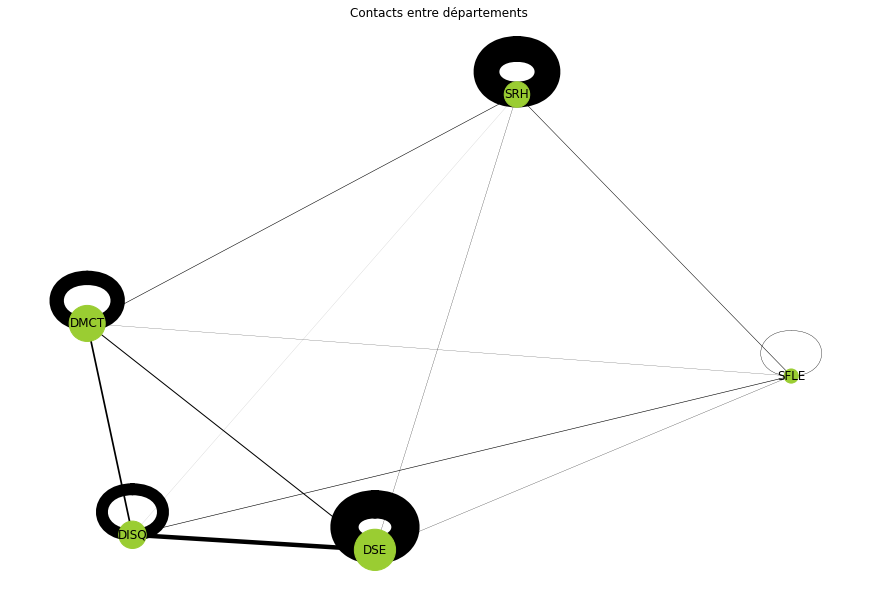
\includegraphics[width=0.65\textwidth]{assets/communaute/communaute_communication_2013.png}
    \caption{Graphes représentant la communication inter et intra départements pour l'année 2013}
    \label{fig:communaute_communication_2013}
\end{figure}

Cependant, en examinant le graphe ci-dessous pour l'année 2015, nous constatons une évolution du nombre de départements, comme mentionné précédemment dans cette section. Cette évolution s'accompagne également d'une évolution de la communication interne au sein des départements. Notamment, le département SFLE, autrefois caractérisé par une communication interne faible, affiche désormais une qualité supérieure. D'autres départements, présents auparavant, ont renforcé leur communication interne. Il est également intéressant de noter que certains départements, autrefois absents, deviennent des éléments presque cruciaux dans la communication. Ils présentent initialement une communication interne très solide, mais développent ensuite des liens interdépartementaux très importants. Par exemple, le département DMI, solide en communication interne, établit également des liens forts avec d'autres départements tels que SFLE, DST, DMCT et DCAR.

\begin{figure}[!h]
    \centering
    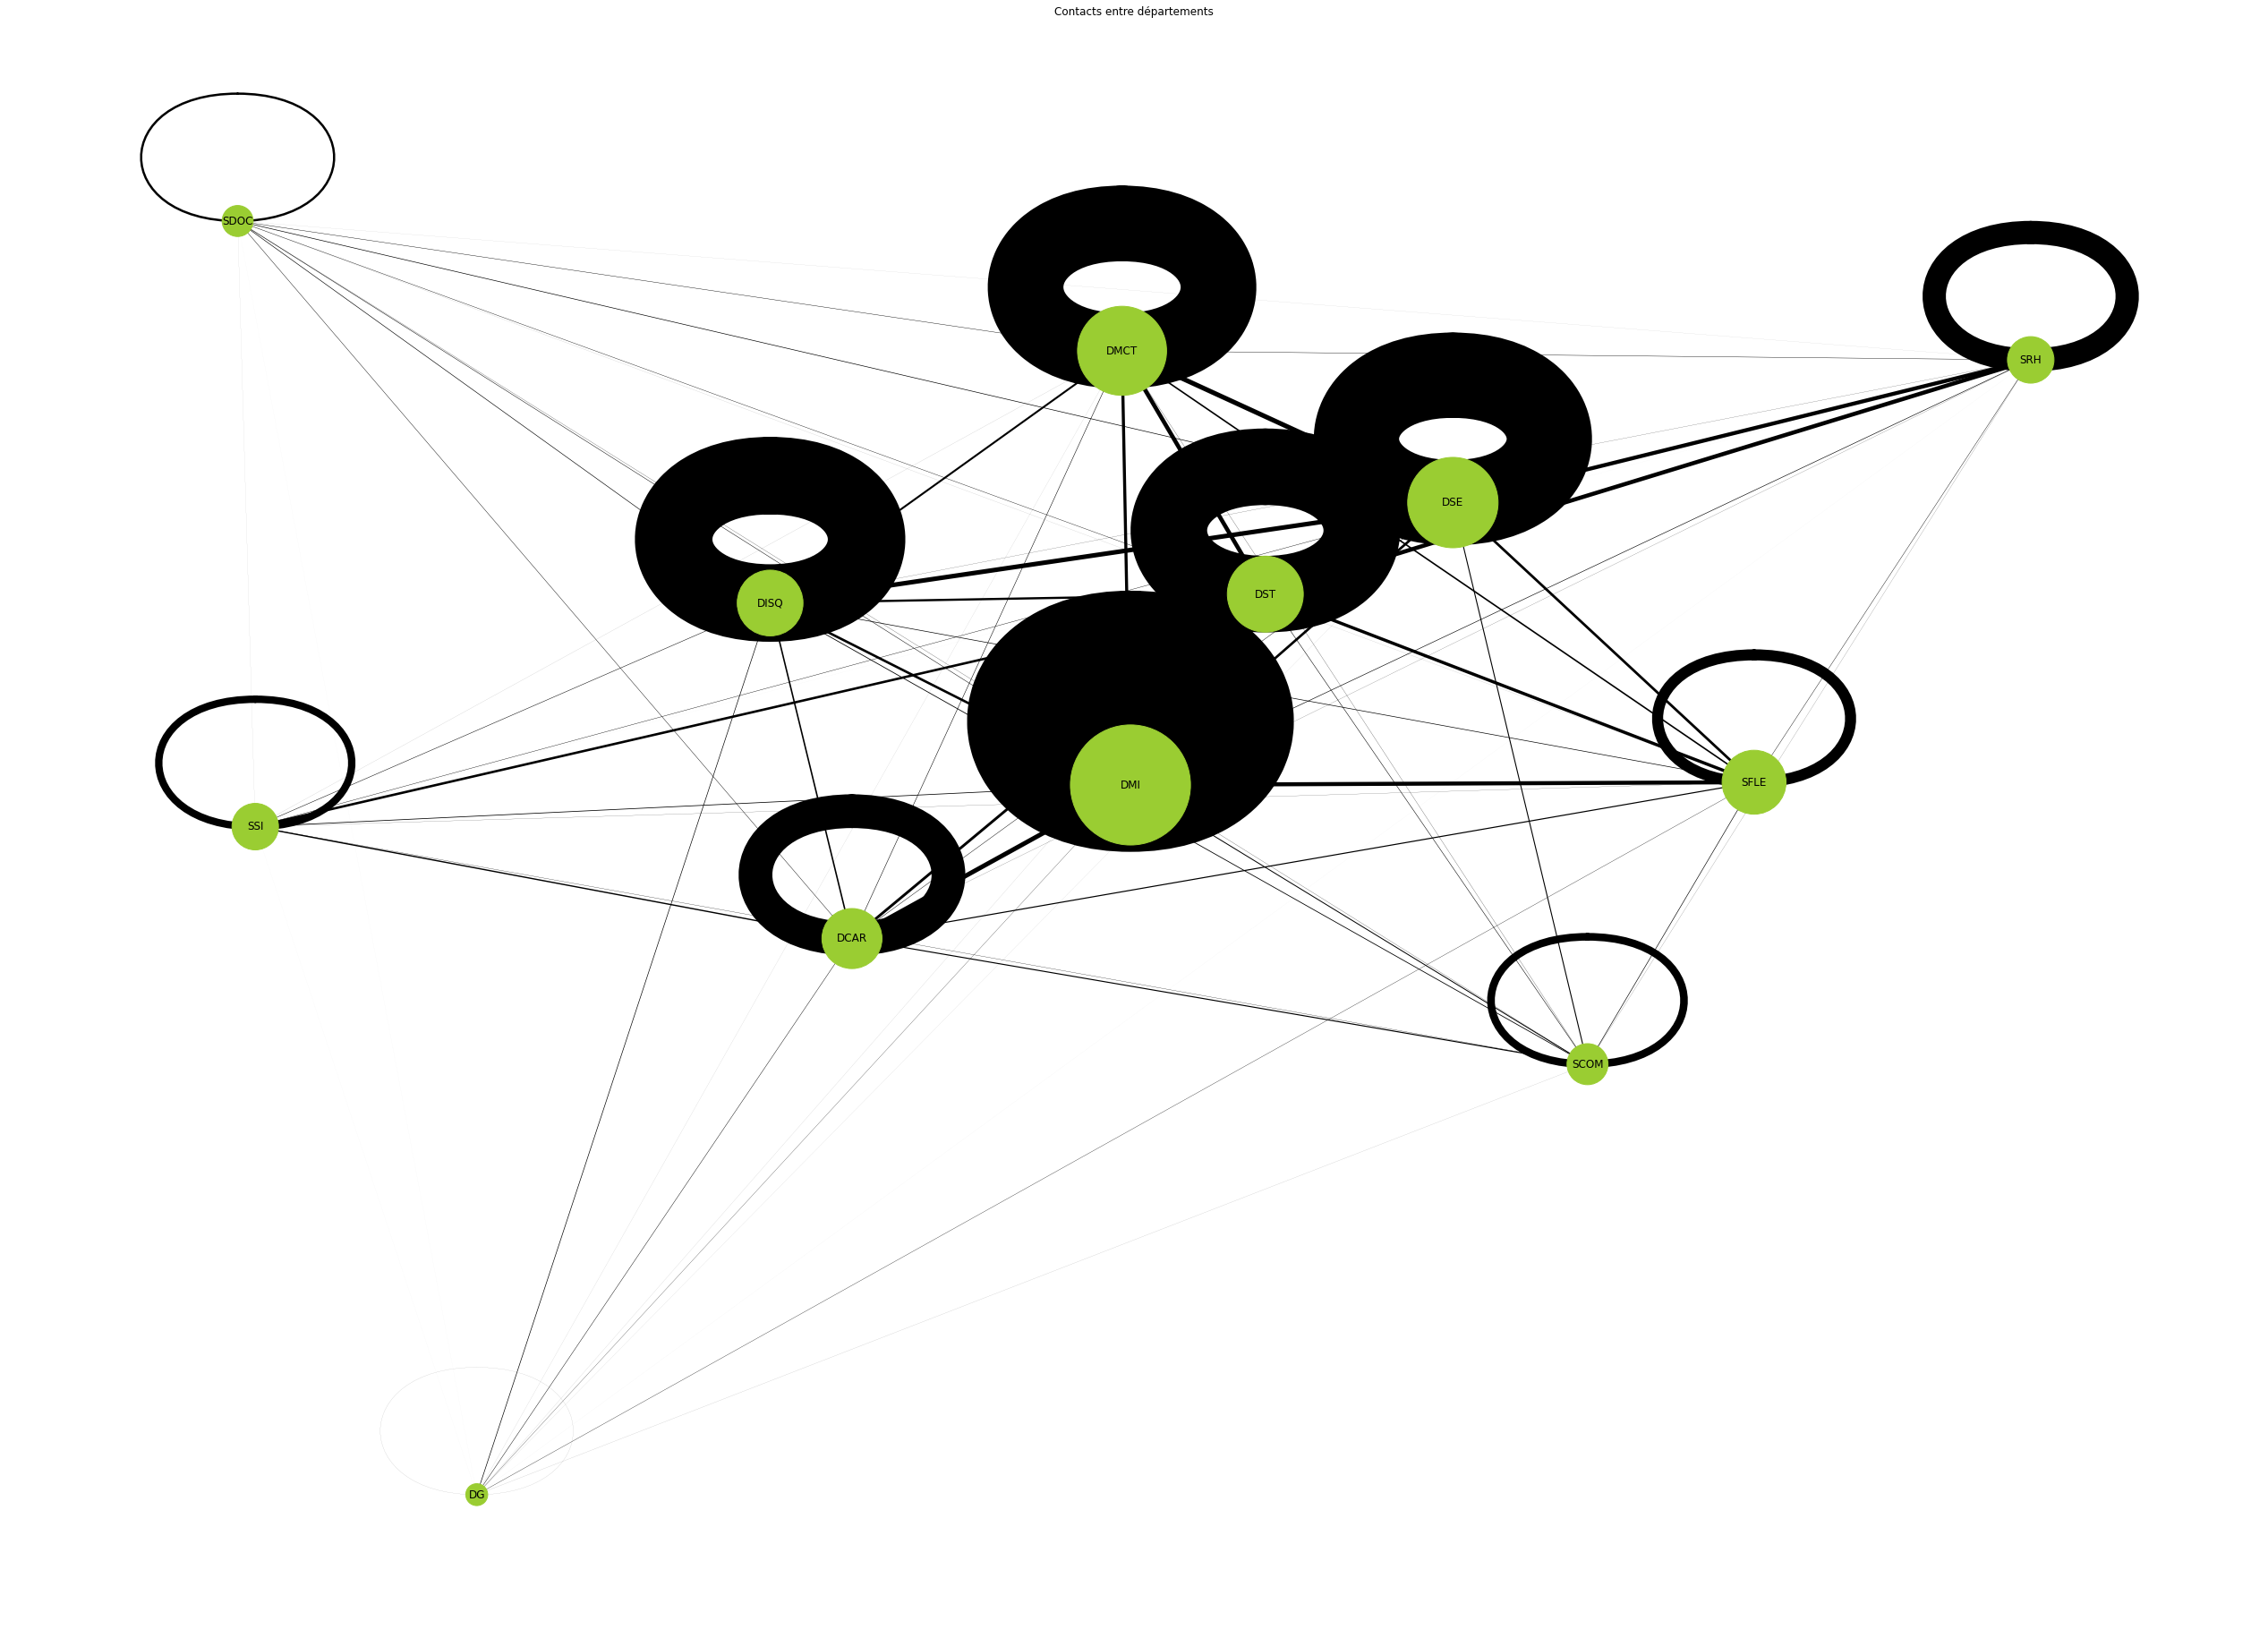
\includegraphics[width=0.65\textwidth]{assets/communaute/communaute_communication_2015.png}
    \caption{Graphes représentant la communication inter et intra départements pour l'année 2015}
    \label{fig:communaute_communication_2015}
\end{figure}

\section{Centralité et Influence}

Dans cette section, nous allons explorer l’importance de certains points dans le graphe en passant par la centralité de ceux-ci au travers du graphe et de ce que cela peut impliquer.

\subsection{Centralité}

En effet, lorsque nous évoquons la centralité, nous faisons référence à la centralité d'intermédiarité entre les différents employés de l'entreprise. Pour illustrer cela, nous avons créé les graphes correspondant aux années 2013 et 2015. \\

Ce graphique de l'année 2013 représente la centralité d'un nœud en fonction du nombres de fois que le noeuds est sur le chemin le plus cours lors de communication sociales avec d'autres employés. Ainsi, les nœuds plus grands et plus foncés correspondent à une centralité plus élevée, comme illustré par le nœud 804, par exemple.

En revanche, dans le graphique de l'année 2015, une diversité de nœuds présentant une centralité importante est observée. En effet, la présence de nœuds très foncés se multiplie.

Nous avons également exploité d'autres graphiques pour confirmer la centralité des points mentionnés précédemment. Nous avons pris en compte diverses mesures telles que la centralité de proximité, la centralité d'intermédiarité, la centralité de vecteur propre, et enfin le coefficient de clustering. Toutes ces mesures semblent converger vers les mêmes résultats.

\begin{figure}[!h]
    \centering
    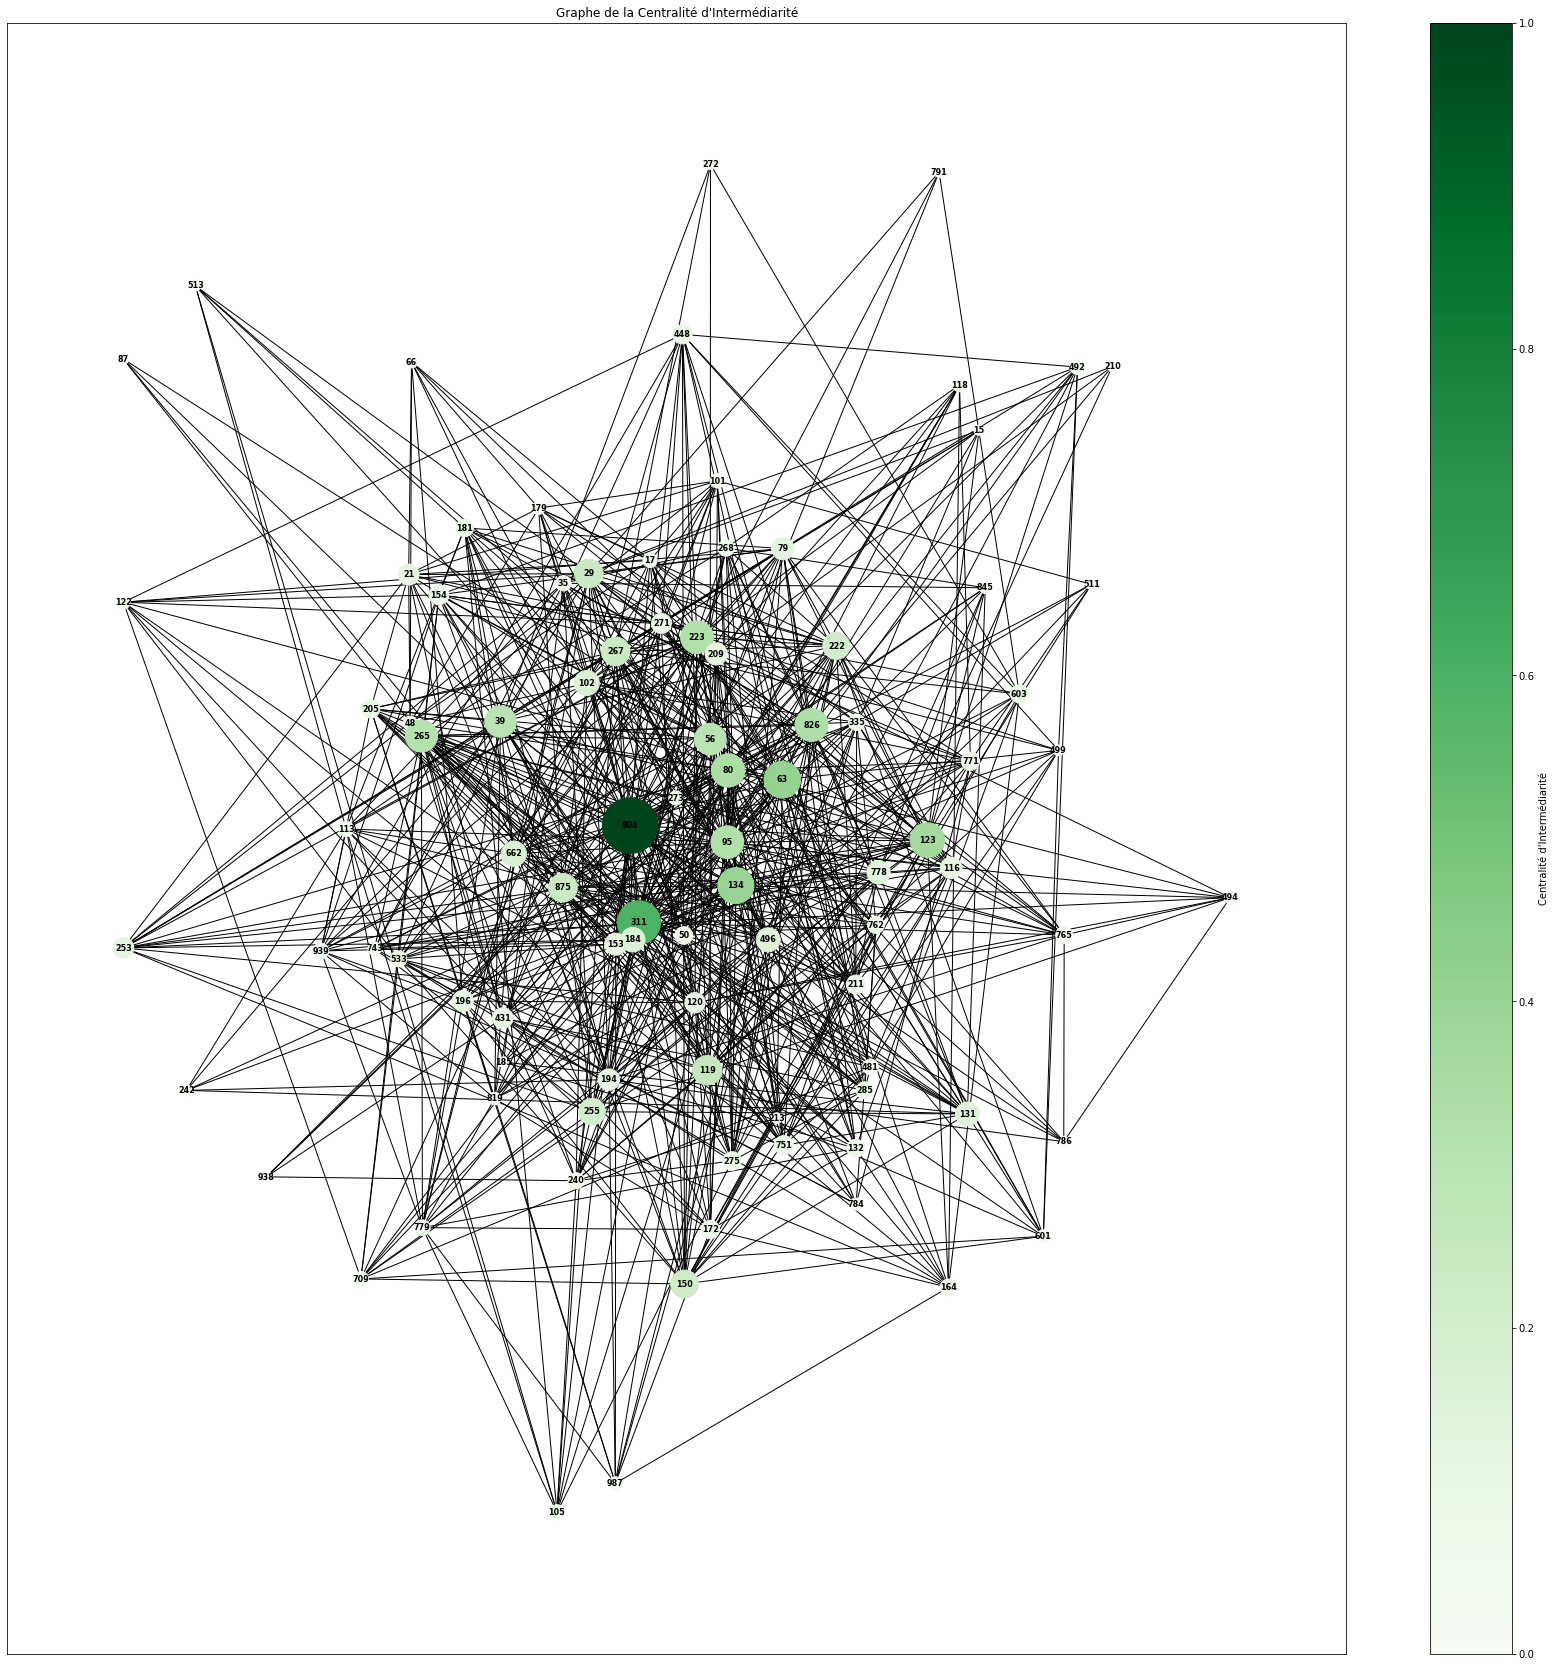
\includegraphics[width=0.45\textwidth]{assets/centralite/between_centralite_2013.png}
    \hfill
    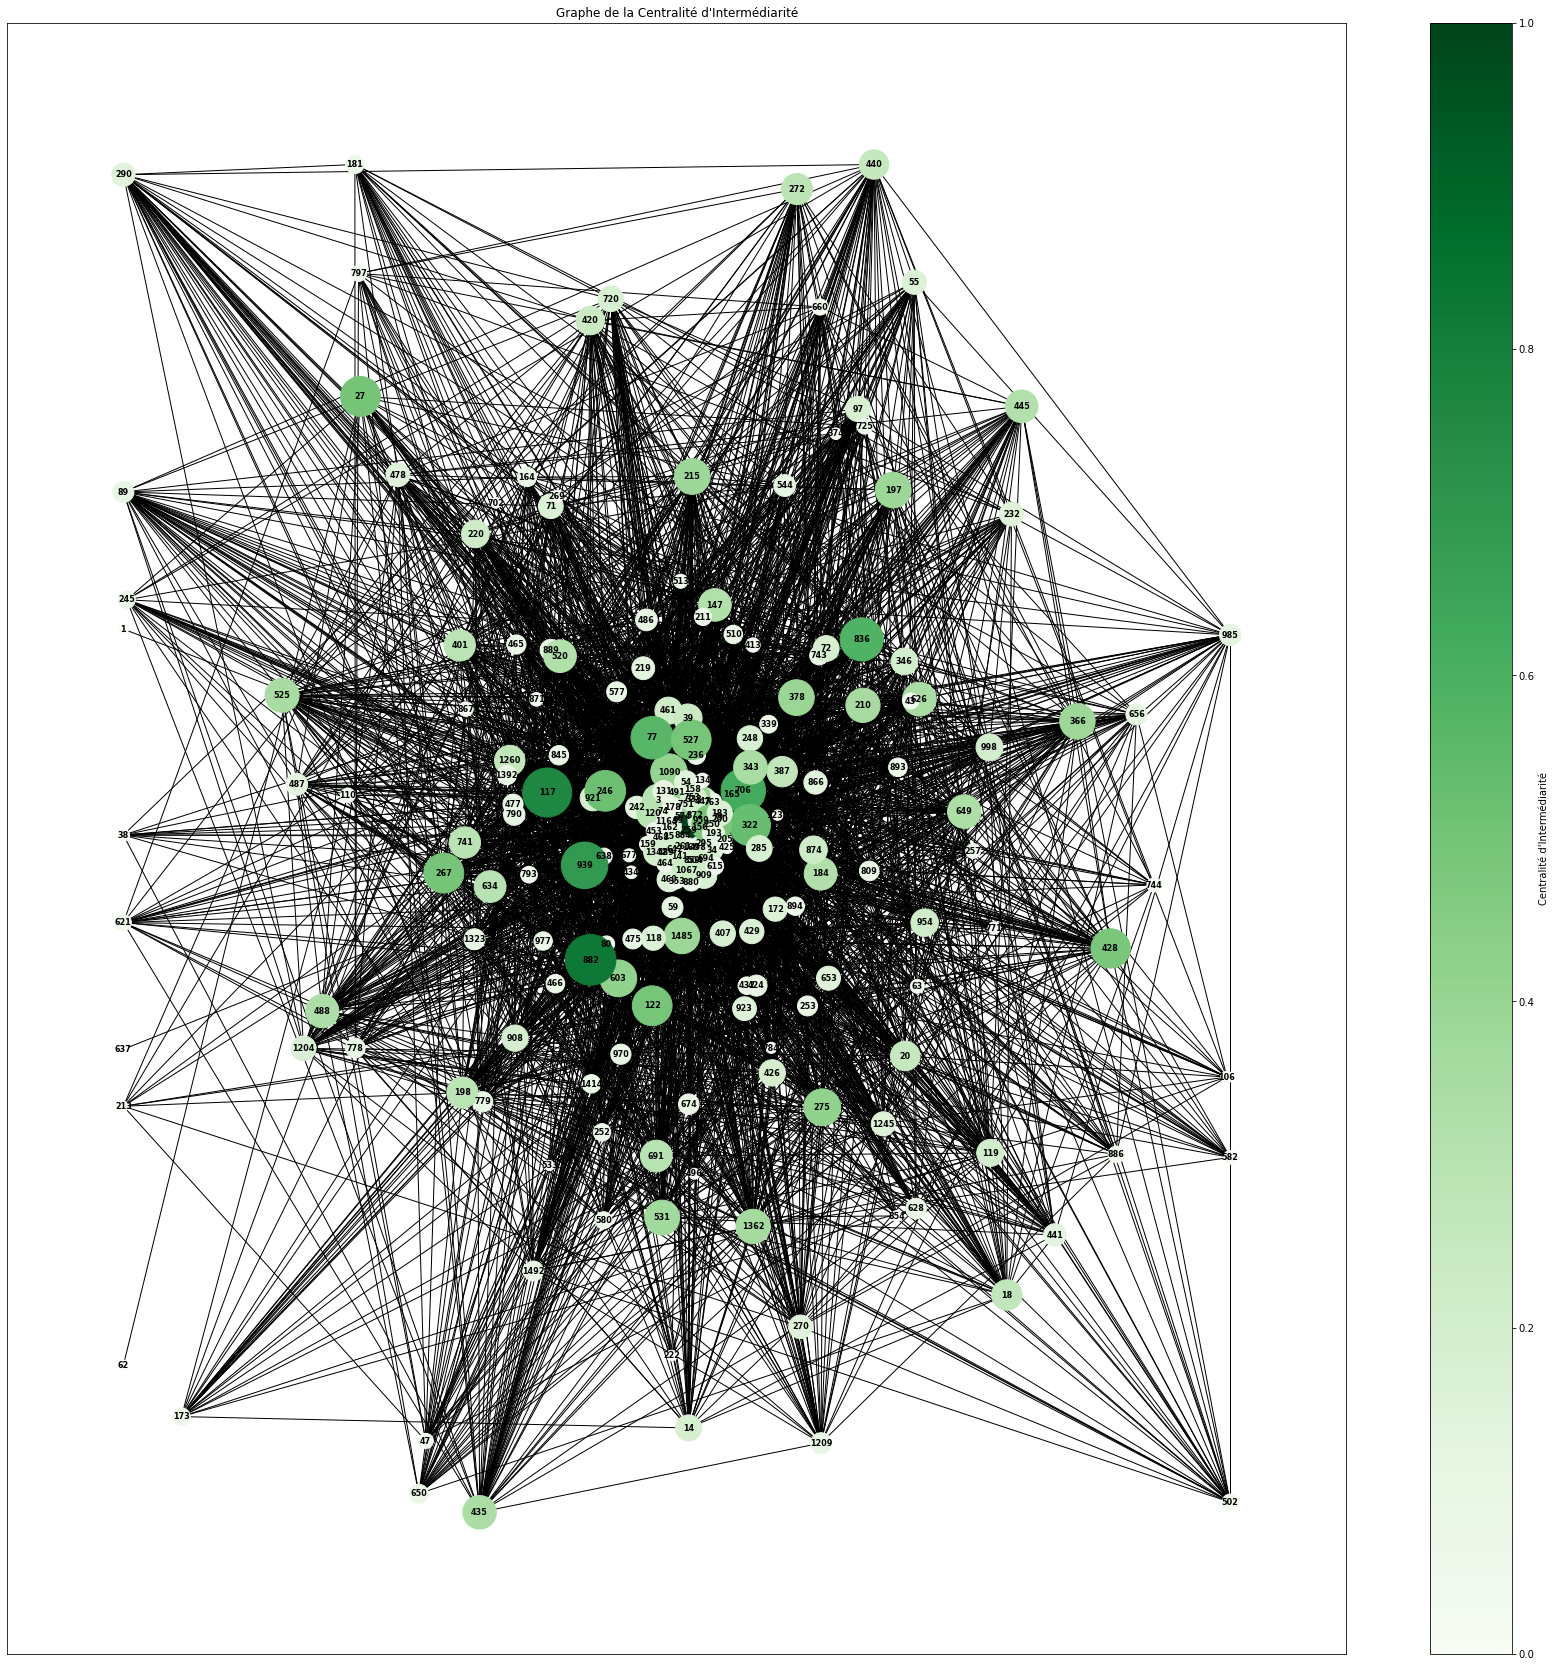
\includegraphics[width=0.45\textwidth]{assets/centralite/between_centralite_2015.png}
    \caption{Graphes représentant la centralité pour les années 2013 et 2015}
    \label{fig:deg_centralite_parallel}
\end{figure}

\subsection{Point de Contrôle}


Dans l’objectif de déterminer les noeuds jouant un rôle important dans la dynamique communicationnel des graphes, nous avons mené une étude sur les noeuds étant ce qu’on appelle un point de contrôle. Effectivement, un point de contrôle est un noeuds stratégique utile pour le contrôle d’information mais aussi pour la prévention de la propagation, dans le cas de notre épidémie évoqué dans une section antérieur, par exemple.

Les analyses antérieures mettent en évidence la centralité de certains nœuds dans la dynamique sociale de l'entreprise. Ces nœuds, au cœur des interactions sociales, semblent correspondre à des postes à haute responsabilité tels que des CEO ou des chefs de projet.

Par conséquent, la circulation des informations se fait principalement à travers ces nœuds centraux. Leur élimination du graphe rendrait la communication au sein de l'entreprise plus complexe, soulignant ainsi leur rôle crucial dans la dynamique communicationnelle.

\section{conclusion}

En conclusion, la réalisation de ce projet nous a permis d’aborder les concepts du cours de « Graph Mining » à travers le sujet de notre choix. Pour réaliser à bien le projet, il nous a été demandé de choisir 2 datasets que nous devions comparer entre eux en utilisant les techniques vues aux cours. Effectivement, notre groupe à décidé de choisir 2 datasets démontrant la communication au sein d’une entreprise. Le premier dataset montre la communication de l’année 2013 et le second dataset montre l’année 2015. 

Durant notre analyse de ce projet, nous avons pu remarquer divers éléments tels que l’importance de certains nœuds insoupçonnés ou alors la présence de sous-population au sein de la population des employés de l’entreprise. 

Ce projet, c’est révélé très enrichissant, car cela nous a permis d’apprendre des techniques que nous n’aurions peut-être jamais utilisées sans ce projet. Effectivement, cela a été très amusant d’effectuer les comparaisons avec des graphes très coloré et très différent de ce que nous utilisons habituellement.


\end{document}
